\documentclass[a4paper]{article} %размер бумаги устанавливаем А4
% \usepackage[T2A]{fontenc}
\usepackage{polyglossia}
\usepackage{url} % добавляем поддержку url-ссылок
\setmainlanguage[babelshorthands=true]{russian} % Язык по-умолчанию русский с поддержкой приятных команд пакета babel
\setotherlanguage{english} % Дополнительный язык = английский (в американской вариации по-умолчанию)
\newfontfamily{\cyrillicfonttt}{Times New Roman}

\usepackage{minted} %пакет для подсветки кода
\usepackage{color}
\usepackage{xcolor} % to access the named colour LightGray
\definecolor{LightGray}{gray}{0.9}
\setdefaultlanguage[forceheadingpunctuation=false]{russian}
% для отступа в первом абзаце
\usepackage{indentfirst} 
\parindent=1.25cm % длина отступа в абзацах
% для продвинутых списков
\usepackage{enumitem} 
\usepackage{amssymb,amsfonts,amsmath,cite,enumerate,float,indentfirst} %пакеты расширений
\usepackage{graphicx}% для вставки картинок
\usepackage{url} % добавляем поддержку url-ссылок
\usepackage{hyperref} % пакет для интеграции гиперссылок
\usepackage{amsmath} % добавляем поддержку математических символов
\usepackage{multirow} % понадобится для создания таблицы с объединенными строками
\usepackage{pdfpages}% Добавление внешних pdf файлов
\usepackage{tocloft}
\renewcommand{\cftsecfont}{\mdseries}
\renewcommand{\cftsecpagefont}{\mdseries}
\cftsetindents{section}{0em}{2em}
\cftsetindents{subsection}{0em}{3em}
\cftsetindents{subsubsection}{0em}{4em}
\renewcommand\cfttoctitlefont{\hfill\normalsize\mdseries}
\renewcommand\cftaftertoctitle{\hfill\mbox{}}
\renewcommand{\cftsecleader}{\cftdotfill{\cftdotsep}}

\usepackage{fontspec}
\setmainfont{Times New Roman} %шрифт 
\graphicspath{{images/}}%путь к рисункам
\usepackage[14pt]{extsizes} % для того чтобы задать нестандартный 14-ый размер шрифта

%\makeatletter
%\renewcommand{\@biblabel}[1]{#1.} % Заменяем библиографию с квадратных скобок на точку:
%\makeatother




\usepackage[tableposition=top]{caption}
\usepackage{subcaption}
\DeclareCaptionLabelFormat{gostfigure}{Рисунок #2}
\DeclareCaptionLabelFormat{gosttable}{Таблица #2}
\DeclareCaptionLabelSeparator{gost}{~–~}
\captionsetup{labelsep=gost}
\captionsetup[figure]{labelformat=gostfigure}
\captionsetup[table]{labelformat=gosttable}
\renewcommand{\thesubfigure}{\asbuk{subfigure}}


\makeatletter

\renewcommand{\section}{\@startsection{section}{1}{0pt}%
                                {-3.5ex plus -1ex minus -.2ex}%
                                {2.3ex plus .2ex}%
{\centering\hyphenpenalty=10000\normalfont\normalsize\mdseries}}

\renewcommand{\subsection}{\@startsection{subsection}{1}{0pt}%
                                {-3.5ex plus -1ex minus -.2ex}%
                                {2.3ex plus .2ex}%
{\centering\hyphenpenalty=10000\normalfont\normalsize\mdseries}}
\renewcommand{\subsubsection}{\@startsection{subsubsection}{1}{0pt}%
                                {-3.5ex plus -1ex minus -.2ex}%
                                {2.3ex plus .2ex}%
{\centering\hyphenpenalty=10000\normalfont\normalsize\mdseries}}
\makeatother


\usepackage{setspace}
% \onehalfspacing % полуторный интервал для всего текста
% или \singlespacing % одиночный интервал для всего текста
% или \doublespacing % двойной интервал для всего текста
\setstretch{1.5} % произвольный интервал

% в тексте
% \begin{onehalfspace}
% фрагмент текста с полуторным межстрочным интервалом
% \end{onehalfspace}
% \begin{doublespace}
% фрагмент текста с двойным межстрочным интервалом
% \end{doublespace}

\sloppy % выравнивание по ширине




%%% Поля и разметка страницы %%%
\usepackage{pdflscape}  % Для включения альбомных страниц
\usepackage{geometry}   % Для последующего задания полей
\geometry{left=3cm}% левое поле
\geometry{right=1.5cm}% правое поле
\geometry{top=2cm}% верхнее поле
\geometry{bottom=2cm}% нижнее поле



\renewcommand{\theenumi}{\arabic{enumi}}% Меняем везде перечисления на цифра.цифра
\renewcommand{\labelenumi}{\arabic{enumi}}% Меняем везде перечисления на цифра.цифра
\renewcommand{\theenumii}{.\arabic{enumii}}% Меняем везде перечисления на цифра.цифра
\renewcommand{\labelenumii}{\arabic{enumi}.\arabic{enumii}.}% Меняем везде перечисления на цифра.цифра
\renewcommand{\theenumiii}{.\arabic{enumiii}}% Меняем везде перечисления на цифра.цифра
\renewcommand{\labelenumiii}{\arabic{enumi}.\arabic{enumii}.\arabic{enumiii}.}% Меняем везде перечисления на цифра.цифра



\newcommand{\imgh}[3]{\begin{figure}[h]\center{\includegraphics[width=#1]{#2}}\caption{#3}\label{ris:#2}\end{figure}}
\newcommand{\imghh}[3]{\begin{figure}[H]\center{\includegraphics[width=#1]{#2}}\caption{#3}\label{ris:#2}\end{figure}}


\usepackage{lastpage}
\usepackage{totcount}
\newcounter{totfigures}
\newcounter{tottables}
\newcounter{totreferences}

\makeatletter
    \AtEndDocument{%
      \addtocounter{totfigures}{\value{figure}}%
      \addtocounter{tottables}{\value{table}}%
	  
      \immediate\write\@mainaux{%
        \string\gdef\string\totfig{\number\value{totfigures}}%
        \string\gdef\string\tottab{\number\value{tottables}}%   

      }%
    }
\makeatother

	

\newcommand{\empline}{\mbox{}\newline}
\newcommand{\likechapterheading}[1]{ 
    \begin{center}
   \MakeUppercase{#1}
    \end{center}
    \empline}



\makeatletter
    \renewcommand{\@dotsep}{2}
    \newcommand{\l@likechapter}[2]{{\@dottedtocline{0}{0pt}{0pt}{#1}{#2}}}
\makeatother
\newcommand{\likechapter}[1]{    
    \likechapterheading{#1}    
    \addcontentsline{toc}{likechapter}{\MakeUppercase{#1}}}


\usepackage{cite} % Красивые ссылки на литературу


%% Список литературы с красной строки (без висячего отступа) %%%
\patchcmd{\thebibliography} %может потребовать включения пакета etoolbox
 {\advance\leftmargin\labelsep}
 {\leftmargin=0pt%
  \setlength{\labelsep}{\widthof{\ }}% Управляет длиной отступа после точки
  \itemindent=\parindent%
  \addtolength{\itemindent}{\labelwidth}% Сдвигаем правее на величину номера с точкой
  \advance\itemindent\labelsep%
 }
 {}{}


\makeatletter
\def\@biblabel#1{#1 }
\makeatother


% настройки цветовой палитры для гиперссылок. Цвета можно на свой вкус выбрать здесь:  https://www.overleaf.com/learn/latex/Using_colours_in_LaTeX
\hypersetup{
    citecolor=gray, % цвет цитирования
    colorlinks=true, 
    linkcolor=black, % цвет для гиперссылок 
    filecolor=magenta, % цвет для ссылок на файл      
    urlcolor=mauve} % цвет для url-ссылок
    \usepackage{listings}

\usepackage{color}
\definecolor{dkgreen}{rgb}{0,0.6,0} 
\definecolor{gray}{rgb}{0.3,0.3,0.3}
\definecolor{mauve}{rgb}{0.42,0,0.92}



\let\bfseries\mdseries 
% грязный хак для удаления жирного текста по всему документу

\usepackage[version=3]{acro}

\DeclareAcroProperty{unit}

\DeclareAcronym{BLE}{ 
    short = {BLE}, 
    long  = {Bluetooth Low-Energy },
	unit = --, 
}

\DeclareAcronym{AFE}{
    short = {AFE},
    long  = {Analog Front End},
	unit = --, 
}

\DeclareAcronym{АЦП}{
  short            = АЦП ,
  long             = Аналого-цифровой преобразователь ,
	unit = --, 
}


\DeclareAcronym{ЭКГ}{
  short            = ЭКГ ,
  long             = Электрокардиограмма ,
  unit = --, 
}

\acsetup{
  make-links,
  list/heading = empty,
  % pages/display = all ,
  pages/fill = {, },
}


\usepackage{longtable,siunitx}

\NewAcroTemplate[list]{physics}{%
  \acronymsmapT{%
    \AcroAddRow{%
      \acrowrite{short}%
      &
      \acrowrite{unit}%
      &
      \acrowrite{list}%
      &
      \acropages
        {\acrotranslate{page}\nobreakspace}%
        {\acrotranslate{pages}\nobreakspace}%
      \tabularnewline
    }%
  }%
  
  
  \acroheading
  \acropreamble
  
  \par\noindent
  \setlength\LTleft{0pt}%
  \setlength\LTright{0pt}%
  
  \begin{longtable}{@{}lll@{\extracolsep{\fill}}l@{}}
    \AcronymTable
  \end{longtable}
}


	
\begin{document}
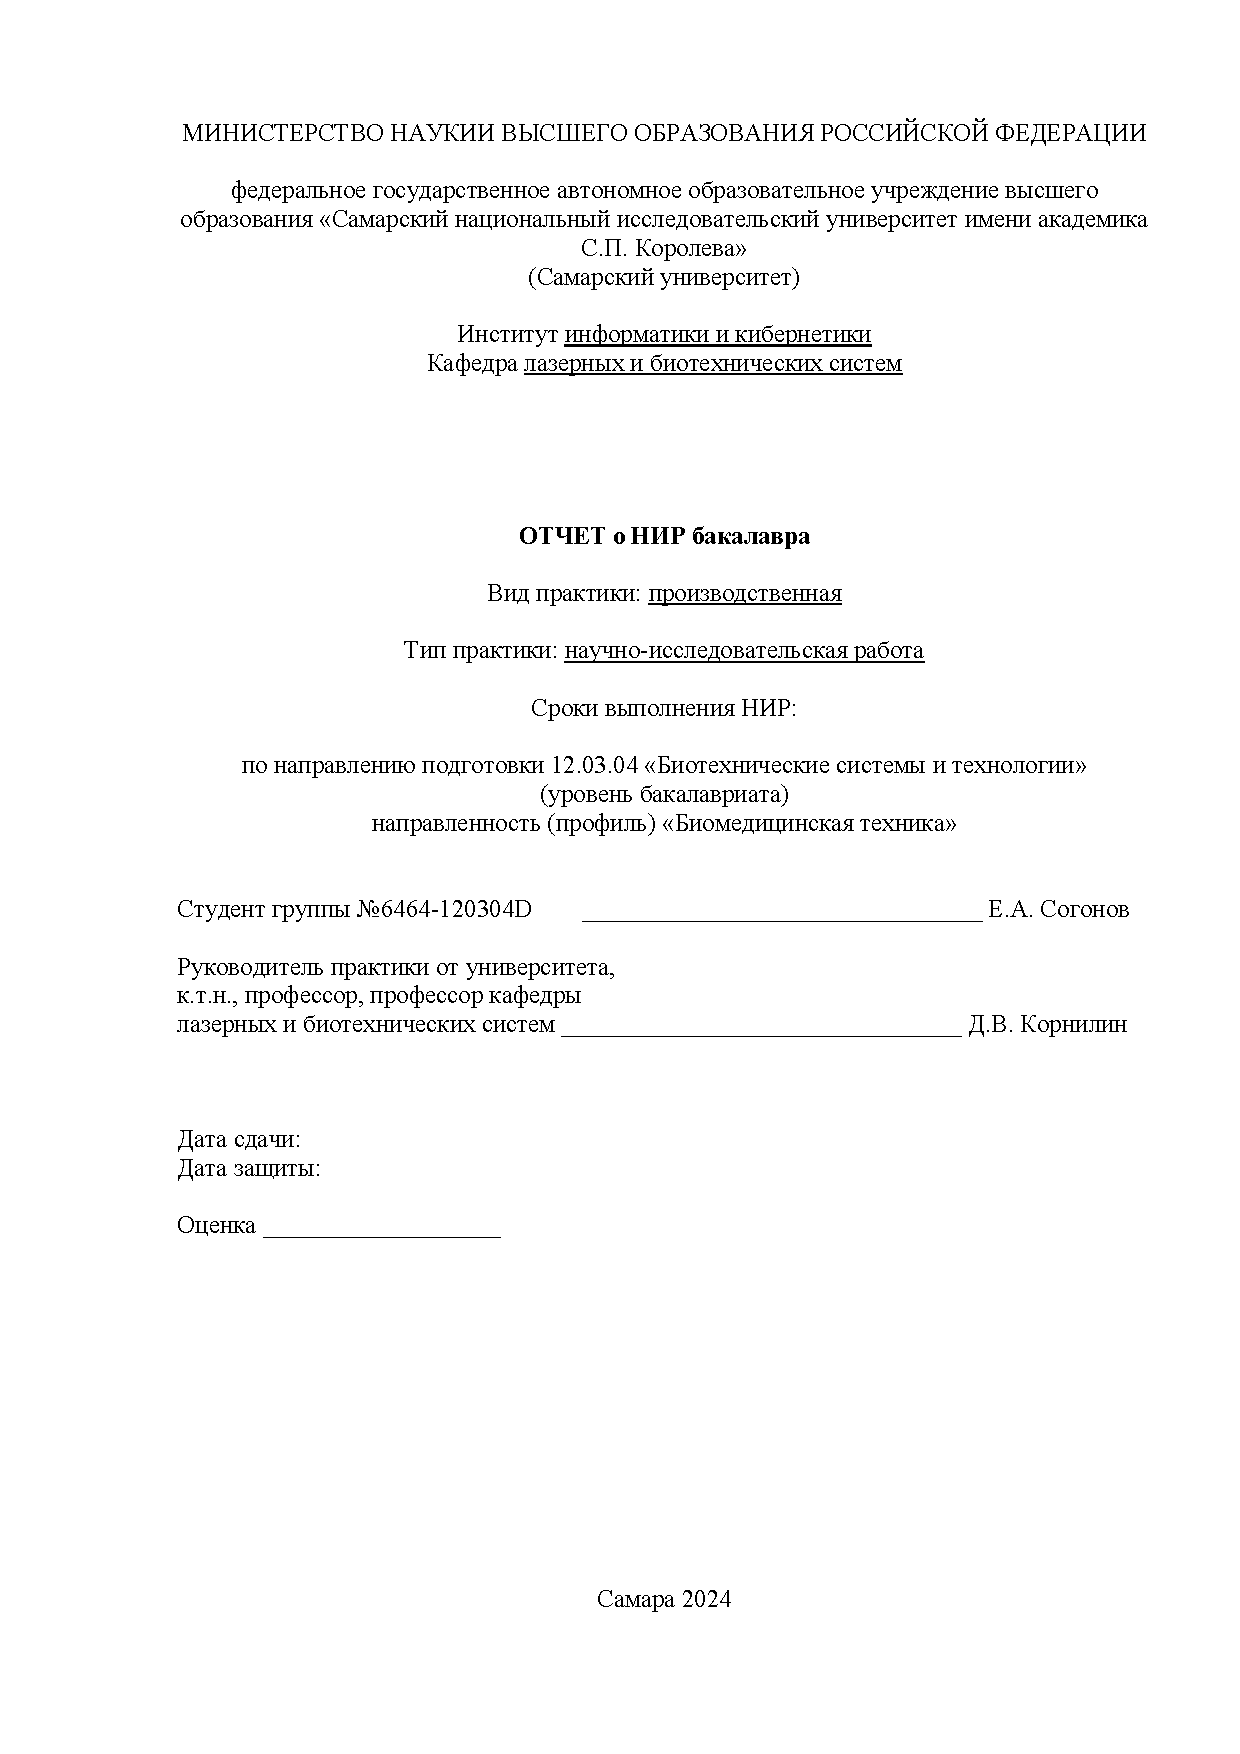
\includepdf[pages={-}]{1.pdf}
\begin{sloppypar} % помогает в кириллическом документе выровнять текст по краям
\newpage % Так добавляется  новая страница



\section{ОПИСАТЕЛЬНАЯ ЧАСТЬ} %Объявили начало раздела

Дерматоскопы, использующие искусственный интеллект для поиска меланомы, представляют собой передовое оборудование для диагностики кожных заболеваний. Используя специальные алгоритмы и искусственный интеллект, они способны обнаруживать изменения в ростках и изменения в пигментации, которые могут быть признаками развития меланомы. Это позволяет врачам более точно и быстро определять вероятность злокачественного образования и принимать соответствующие меры. В результате, ранняя диагностика меланомы может спасти жизни пациентов и повысить эффективность лечения этого опасного заболевания.

\section{Обзор аналогов} %Объявили начало раздела


Некоторые из производителей дерматоскопов, использующих искусственный интеллект для поиска меланомы, включают:
- FotoFinder Systems, Inc.
- 3Gen
- Illuco Corporation
Каждая из этих компаний создает передовые дерматоскопы с различными функциями и алгоритмами искусственного интеллекта для более точной диагностики меланомы и других кожных заболеваний.

Рассмотрим эти примеры подробнее.
\subsection{ FotoFinder Moleanalyzer Pro AI}
Moleanalyzer Pro AI \cite{vexia} - это передовая дерматоскопическая система, разработанная компанией FotoFinder Systems, Inc. Она представляет собой инновационное медицинское оборудование, которое использует искусственный интеллект для диагностики кожных заболеваний, включая меланому.

Moleanalyzer Pro AI обладает специальными алгоритмами, которые способны анализировать изображения родинок и образований на коже с высокой точностью. Благодаря использованию искусственного интеллекта, система способна обнаруживать даже самые маленькие изменения в образованиях, что делает диагностику меланомы более эффективной и точной.

Moleanalyzer Pro AI также обладает возможностью сравнения изображений течения времени, что позволяет врачам отслеживать изменения в образованиях на коже и более точно оценивать их риск развития меланомы.

Эта передовая система является важным инструментом для врачей дерматологов в диагностике и мониторинге кожных заболеваний, что в конечном итоге позволяет более раннее выявление меланомы и улучшение результатов лечения.

Важно отметить, что  система отличается высокая стоимостью(~10млн руб), низкой мобильностью(представляет собой целый компьютерный комплекс).


\subsection{3Gen DermLite HUD}

3Gen DermLite HUD\cite{drmlt} (Heads-Up Display) - это инновационное дерматоскопическое устройство, предназначенное для диагностики кожных заболеваний. Основным преимуществом данного устройства является возможность отображения изображений прямо на голове  с помощью специального гарнитура. Это позволяет врачам более удобно и точно исследовать кожу пациента, обращая внимание на изменения в ростках и образованиях.

DermLite HUD оснащен различными режимами освещения и увеличения, что позволяет профессионалам в области дерматологии получить детальные изображения кожи пациента. Устройство также может быть использовано для захвата изображений и последующего хранения и анализа, что облегчает мониторинг изменений в заболеваниях кожи.

3Gen DermLite HUD предоставляет врачам инструмент для более точной диагностики и мониторинга кожных заболеваний, что в итоге способствует раннему выявлению и эффективному лечению различных патологий.

Данное устройство отличается тем, что является достаточно мобильным и недорогим.



\subsection{Illuco IDS-1000 }
 
Дерматоскоп Illuco IDS-1000  \cite{IDS}  был разработан специалистами ILLUCO optical, у него превосходные оптические и световые характеристики:
10-кратное увеличение
Контактная и бесконтактная дермоскопия с поляризованным светом
Контактная и бесконтактная дермоскопия с неполяризованным светом
Совместимость со смартфонами и камерами (только IDS-1000 Plus)



Достаточно маленький для кармана или ручной сумки
Идеально подходит для непрофессионалов, которые хотят лично наблюдать за изменениями своей кожи
Разумная цена
Для проведения дерматоскопии требуется высококачественная увеличительная линза, а также высококачественные источники света, которые помогут вам исследовать структуры и узоры кожи.

Большинство описанных моделей еще не используют искусственный интеллект для выдачи диагноза, кроме Moleanalyzer Pro AI, который достаточно дорог и не является портативным. 

Целью создания нашего устройства является создание дерматоскопа, имеющего компактный размер, и способного провести первичный анализ изображений кожи прямо на устройстве. Так же оно должно  сохранять снимки на внешний накопитель(SD-карта или FLASH-накопитель), и передавать их на ПК/смартфон.

\section{Структурная схема устройства} %Объявили начало раздела


\end{sloppypar}
% это титульный лист

% \input{tex/01_title}% это титульный лист
% \input{tex/02_task}% это задание
% \begin{sloppypar} % помогает в кириллическом документе выровнять текст по краям
\newpage % Так добавляется  новая страница
\section*{РЕФЕРАТ} %Объявили начало раздела

Пояснительная записка: \pageref*{LastPage}~страниц, \totfig~рисунков, источников, 1 приложение.\\

 % \tottab~таблиц...
 
 
 
ГЛЮКОЗА, УСТРОЙСТВО СЧИТЫВАНИЯ ДАННЫХ, МИКРОКОНТРОЛЛЕР, BLUETOOTH, STM32WB55RCV6


В курсовом проекте разработаны структурная и принципиальная схемы устройства считывания данных для непрерывного мониторинга уровня глюкозы, осуществлен выбор микроконтроллера c интегрированным блоком Bluetooth и АЦП. Разработан алгоритм анализа данных и реализующая его программа на языке Си.

% возможно добавим еще каких то фраз

\end{sloppypar}
% это реферат
% \newpage
\renewcommand{\contentsname}{СОДЕРЖАНИЕ}
{\renewcommand{\baselinestretch}{1.5} %интервал для содержания
\tableofcontents
       
}% это содержание
% \begin{sloppypar} % помогает в кириллическом документе выровнять текст по краям
\newpage % Так добавляется  новая страница
\section*{ВВЕДЕНИЕ} %Объявили начало раздела
Диабет превратился в одну из основных эпидемий здравоохранения современной эпохи. Ожидается, что во всем мире общее число людей с диабетом вырастет со 171 миллиона в 2000 году до 366 миллионов в 2030 году.\cite{ADXL}

Мало того, что диабет был шестой по значимости причиной смерти, указанной в свидетельствах о смерти в США в 2020 году, но предполагаемая стоимость диабета в Соединенных Штатах в 2002 году составила 132 миллиарда долларов, включая как прямые, так и косвенные расходы (инвалидность, инвалидность, потеря работы, преждевременная смертность).

Известно, что строгий гликемический контроль снижает разрушительные и дорогостоящие вторичные микро- и макрососудистые осложнения, связанные с диабетом, тем самым улучшая качество жизни миллионов пациентов с диабетом и значительно сокращая расходы на здравоохранение. Также, строгий контроль уровня глюкозы обеспечивает клинические преимущества у пациентов в критическом состоянии.


Непрерывный мониторинг глюкозы(НМГ) -- метод регистрации изменений концентрации глюкозы в крови, при котором результаты измерений фиксируются не реже чем каждые 5 мин на протяжении длительного времени (более суток). Применяемые в настоящее время устройства для НМГ позволяют получить данные о гликемии косвенно по концентрации глюкозы в межтканевой жидкости.

В данном курсовом проекте  рассматривается способ создания устройства на базе микроконтроллера, который сможет отслеживать уровень глюкозы в крови человека.  В процессе были подобраны необходимые в задании микроконтроллер с интегрированным модулем Bluetooth, акселерометр, а также написана управляющая программа на языке Си. 



\end{sloppypar}
% это введение
\begin{sloppypar} % помогает в кириллическом документе выровнять текст по краям
\newpage % Так добавляется  новая страница
\section{РАЗРАБОТКА СТРУКТУРНОЙ СХЕМЫ УСТРОЙСТВА} %Объявили начало раздела

% Многие эксперты и исследователи пытались разработать неинвазивные глюкометры. Однако в настоящее время неинвазивное определение уровня глюкозы в крови все еще имеет проблемы, такие как чувствительность и сигналы фонового шума, которые необходимо преодолеть, а использование защитных покрытий, таких как pHEMA \cite{Ph}, может обеспечить минимально инвазивное и точное измерение изменений уровня глюкозы в крови.

% Таким образом, основной целью данного исследования является достижение точного и эффективного измерения уровня глюкозы в крови у пациентов с диабетом, а также уменьшение боли и дискомфорта во время процесса, что может улучшить качество жизни. Мы разрабатываем электрохимический датчик на основе массива микроигл, модуль схемы обнаружения глюкозы и модуль передачи для размещения в носимом устройстве, которое может непрерывно определять концентрацию глюкозы в интерстициальной жидкости [ISF] с низкой инвазивностью и передавать данные на мобильный телефон по Bluetooth, с точным измерением изменений концентрации глюкозы. Минимально инвазивная рана после использования показана на \ref{ris:Figures/struct2.png}. 
% \imghh{150mm}{Figures/struct2.png}{Минимально инвазивная рана после использования CGMS, эта небольшая рана практически не вызывает боли и кровотечения}


% Концепция микропереноса была применена для переноса глюкозооксидазы на датчик матрицы микроигл. Этот набор микроигл был приобретен у RichHealth Technology. Датчик массива микроигл показан на рисунке  \ref{ris:Figures/struct1.png}., который включает в себя три части: рабочий электрод (WE), противоэлектрод (CE) и электрод сравнения (RE). Массив микроигл изготовлен из нержавеющей стали SUS316L с использованием процесса штамповки металла. Каждая микроигла имеет длину 1 мм, ширину 0,25 мм и толщину 0,1 мм. Затем противоэлектрод покрывают золотом, рабочий электрод покрывают золотом и ПАНИ, а электрод сравнения покрывают Ag/AgCl. Каждый массив WE имеет площадь 3 мм×3 мм и состоит из 3×4 микроиглы. Рабочая площадь каждого массива микроигл составляет около 1,2 мм.2. Все иглы скошены для предотвращения нестабильности сигнала из-за отслоения глюкозооксидазы при прокалывании под кожей


% \imghh{150mm}{Figures/struct1.png}{Структура датчика матрицы микроигл;}


Структурная схема устройства представлена на рисунке \ref{ris:Figures/struct.png}.
\imghh{150mm}{Figures/struct.png}{Структурная схема устройства}


Принцип работы устройства заключается в следующем: микроконтроллер управляет подсветкой и камерой. С помощью камеры получаем изображение кожи, которое будет обработано посредством нейросети внутри микроконтроллера. Питается вся система с помощью встроенного аккумулятора, также предусмотрено питание/заряд аккумулятора от USB, с помощью внешнего блока питания или от порта ПК. 

Результаты анализа выводятся на ЖК-экран. Снимки кожи и результаты их обработки передаются по внешнему модулю Bluetooth, подключенному к микроконтроллеру, и могут быть записаны во Flash-накопитель или SD-карту для дальнейших исследований.


\end{sloppypar}
% это раздел структурной схемы
% \begin{sloppypar} % помогает в кириллическом документе выровнять текст по краям
\newpage % Так добавляется  новая страница
\section{РАЗРАБОТКА ПРИНЦИПИАЛЬНОЙ СХЕМЫ УСТРОЙСТВА} %Объявили начало раздела


\subsection{Выбор усилителя биопотенциалов}
Схема подает напряжение, чтобы вызвать окислительно-восстановительную реакцию на рабочем электроде. Этот заряд усиливает токовую реакцию электрода, и, наконец, чувствительная схема усиливает сигнал электрода. Противоэлектрод (CE) находится под отрицательным напряжением относительно рабочего электрода. Кроме того, ток, генерируемый на выводе рабочего электрода, составляет менее 100 нА при концентрации мг/дЛ. Поскольку этого тока недостаточно, для преобразования тока в выходное напряжение требуется трансимпендансный усилитель на операционном усилителе с чрезвычайно низким током смещения. Его схема показана на  рисунке \ref{ris:Figures/struct-tr.png}. 
\imghh{80mm}{Figures/struct-tr.png}{Трансимпедансный усилитель}



С этой целью мы использовали операционный усилитель MAX9913 \cite{MAX9913}, который подходит для аналогичных применений. При комнатной температуре имеет низкий ток смещения и хорошие характеристики защиты от шумовых помех. Типичная схема работы инструментального усилителя из даташита MAX9913 приведена на рисунке  \ref{ris:Figures/max.png}. 
\imghh{80mm}{Figures/max.png}{Cхема включения MAX9913}

Нумерация и назначение выводов MAX9913 приведено ниже (рисунки \ref{ris:Figures/max1.png}, \ref{ris:Figures/max2.png}).
\imghh{80mm}{Figures/max1.png}{Распиновка MAX9913}

\imghh{150mm}{Figures/max2.png}{Назначение выводов MAX9913}




\subsection{Выбор микроконтроллера}
С учетом технического задания микроконтроллер должен обладать следующими свойствами:
\begin{onehalfspace}
	\begin{itemize}
		\item[--]Интерфейс для работы с термодатчиком :  $I^2$C;
		\item[--]Интерфейс для работы с внешней флеш-памятью: SPI или $I^2$C;
		\item[--]Для передачи данных по Bluetooth: встроенный стек протокола Bluetooth;
		\item[--]Малое энергопотребление;
	\end{itemize}
\end{onehalfspace}

Для решения задачи был выбран микроконтроллер STM32WB55RCV6 фирмы ST Microelectronics \cite {STM}.STM32WB55 содержит два производительных ядра ARM-Cortex:
\begin{onehalfspace}
	\begin{itemize}
		\item[--] ядро ARM® -Cortex® M4 (прикладное), работающее на частотах до 64 МГц, для пользовательских задач имеется модуль управления памятью, модуль плавающей точки, инструкции ЦОС (цифровой обработки сигналов), графический ускоритель (ART accelerator);
		\item[--] ядро ARM®-Cortex® M0+ (радиоконтроллер) с тактовой частотой 32 МГц, управляющее радиотрактом и реализующее низкоуровневые функции сетевых протоколов;
	\end{itemize}
\end{onehalfspace}


Основные характеристики:
\begin{onehalfspace}
	\begin{itemize}
		\item[--] типовое энергопотребление 50 мкА/МГц (при напряжении питания 3 В);
		\item[--] потребление в режиме останова 1,8 мкА (радиочасть в режиме ожидания (standby));
		\item[--] потребление в выключенном состоянии (Shutdown) менее 50 нА;
		\item[--] диапазон допустимых напряжений питания 1,7…3,6 В (встроенный DC-DC–преобразователь и LDO-стабилизатор);
		\item[--] рабочий температурный диапазон -40…105°С.
	\end{itemize}
\end{onehalfspace}


Структурная схема микроконтроллера приведена на рисунке \ref{ris:Figures/stm32.png}, а назначение выводов портов корпуса на рисунке \ref{ris:Figures/stm32io.png}.

\imghh{90mm}{Figures/stm32io.png}{Назначение выводов}


\imghh{110mm}{Figures/stm32.png}{Структурная схема}


Подключение будет осуществляться согласно типовой схеме из Application note\cite {STM_an}(рисунок \ref{ris:Figures/stm32an.png}).
\imghh{160mm}{Figures/stm32an.png}{Типовая схема подключения STM32WB55}






\begin{sloppypar} % помогает в кириллическом документе выровнять текст по краям


\subsection{Выбор встроенного носителя}
 В качестве носителя информации выберем последовательную FLASH-память серии W25Q \cite{W25Q}. Данная последовательная память может быть различной ёмкости — 8, 16, 32, 64, 128, 256 Мбит и т. д. Подключается такая память по интерфейсу SPI, а также по многопроводным интерфейсам Dual SPI, Quad SPI и QPI. Мы подключим данную микросхему по обычному интерфейсу SPI.
Необходимый объем памяти для наших нужд рассчитывается по формуле: объем памяти= 16*1*60*24 = 23040bit \approx 23 Mbit
где 16 - необходимый объем памяти для хранения одного измерения в битах, 1- число измерений в минуту, 60 - количество минут в одном часе, 24 - количество часов в сутках.
Таким образом, для хранения данных в течение 24 часов нам нужно выбрать FLASH-память с ёмкостью 32 Mbit.

 
 
 

Краткие основные характеристики W25Q:

\begin{onehalfspace}
	\begin{itemize}
		\item[--]Потребляемая мощность и температурный диапазон:
		\item[--]Напряжение питания 2.7…3.6 В
		\item[--]Типичный потребляемый ток: 4 мА (активный режим), <1 мкА (в режиме снижения мощности)
		\item[--]Рабочий температурный диапазон -40°C…+85°C.
	\end{itemize}
\end{onehalfspace}

Гибкая архитектура с секторами размером 4 кбайт:
\begin{onehalfspace}
	\begin{itemize}
		\item[--]Посекторное стирание (размер каждого сектора 4 кбайт)
		\item[--]Программирование от 1 до 256 байт
		\item[--]До 100 тыс. циклов стирания/записи
		\item[--] 20-летнее хранение данных
	\end{itemize}
\end{onehalfspace}


Максимальная частота работы микросхемы:
\begin{onehalfspace}
	\begin{itemize}
		\item[--]104 МГц в режиме SPI
		\item[--]208/416 МГц — Dual / Quad SPI
	\end{itemize}
\end{onehalfspace}

Также микросхема существует в различных корпусах, но в большинстве случаев распространён корпус SMD SO8. Распиновка микросхемы следующая(рисунок \ref{ris:Figures/w25io.png}).
\imghh{90mm}{Figures/w25io.png}{Распиновка W25Q32}

Описание выводов из  \cite {W25Q}(рисунок \ref{ris:Figures/w25qan.png}).
\imghh{160mm}{Figures/w25qan.png}{Описание выводов W25Q32}
К микроконтроллеру подключается по стандартному интерфейсу SPI.



\end{sloppypar}
 



\begin{sloppypar} % помогает в кириллическом документе выровнять текст по краям


\subsection{Выбор встроенного носителя}
Для точного измерения температуры окружающей среды (в том числе места контакта устройства с телом исследуемого) возникла необходимость установки периферийного высокоточного датчика, который обеспечивал бы схему информацией о температуре и в случае перегрева предпринимались бы необходимые меры для исключения снятия неточных данных. Таковым был выбран датчик от фирмы Texas Instruments TMP102 \cite{TMP102}. Типовая схема включения и конфигурация выводов изображены на рисунках \ref{ris:Figures/tmpcnct.png}  и \ref{ris:Figures/tmp.png}. Информацию с него будем получать по шине $I^2$C

Также микросхема существует в различных корпусах, но в большинстве случаев распространён корпус SMD SO8.
\imghh{90mm}{Figures/tmpcnct.png}{Типичная схема включения TMP102}

\imghh{160mm}{Figures/tmp.png}{Описание выводов и распиновка TMP102}
К микроконтроллеру подключается по стандартному интерфейсу $I^2$C.





\end{sloppypar}
 


\subsection{Схема питания}
Питание данного устройства спроектировано от часовой батарейки с напряжением питания 1.5В. В связи с тем, что практически все элементы схемы требуют напряжение питания больше 3 вольт, используем повышающий DC-DC преобразователь напряжения. Возьмем модель от Texas Instruments TPS63802 2-A\cite{TPS63802}. Конфигурация выводов изображена на рисунке \ref{ris:Figures/TPS63802.png}. Данный конвертер поднимет напряжение с 1.8 вольт до 3.5. 


\imghh{160mm}{Figures/TPS63802.png}{Распиновка и описание выводов TPS63802}

В целях обеспечения сохранности первоначального вида сигнала, поставим LOW-DROP-OUT регулятор напряжения перед питанием усилителя биопотенциалов. 

Возьмем R1517S331D-E2-FE от компании RICOH[3]. На рисунке \ref{ris:Figures/r15.png} показано типичное включение данного регулятора в цепь. Данный регулятор обезопасит усилитель от дребезгов питания.


\imghh{120mm}{Figures/r15.png}{Типовая схема включения R1517S331D}










\end{sloppypar}
% это раздел принципиальной схемы
% \begin{sloppypar} % помогает в кириллическом документе выровнять текст по краям
\newpage % Так добавляется  новая страница
\section{РАЗРАБОТКА ПРОГРАММЫ} %Объявили начало раздела

Алгоритм начинается с включения питания и инициализации всех периферийных устройств и модулей. запуск тактирования, инициализация портов ввода-вывода, таймеров, аналого-цифрового преобразователя,  инициализация интерфейсов SPI и $I^2$C, а так же периферия, необходимая стеку Bluetooth. Далее инициализируется модули, подключенные к микроконтроллеру - термодатчик, flash память и Bluetooth. 

После этого начинается основная программа. по таймеру запускается АЦП, получающий сигнал с усилителя биомпедансов. По готовности данных срабатывает прерывание, в обработчике которого происходит запись данных из регистров АЦП в буферный массив. При наполенении массива происходит запись страницы памяти на FLASH память.  Массив данных передается по Bluetooth и записывается на карту памяти. Основная программа возвращается на начало своего цикла. 

\end{sloppypar}
% это раздел принципиальной схемы
% \begin{sloppypar} % помогает в кириллическом документе выровнять текст по краям
\newpage % Так добавляется  новая страница

\section*{ЗАКЛЮЧЕНИЕ} %Объявили начало раздела
\addcontentsline{toc}{section}{ЗАКЛЮЧЕНИЕ}

В данном курсовом проекте рассмотрены принципы разработки устройств на базе микроконтроллеров. Был разработано устройство для непрерывного мониторинга уровня глюкозы. Данные передаются по интерфейсу Bluetooth и записываются на карту памяти. В процессе работы были разработаны структурная и принципиальная схемы устройства, были проведены необходимые расчёты для получения заданной погрешности, осуществлен выбор микроконтроллера и вспомогательных компонентов схемы. 



\end{sloppypar}
% это заключение
\newpage
\renewcommand\refname{\centering СПИСОК ИСПОЛЬЗОВАННЫХ ИСТОЧНИКОВ}
\begin {thebibliography} {99}

\bibitem {vexia}FotoFinder Moleanalyzer pro [Электронный ресурс]. URL: \href{https://www.fotofinder.de/en/technology/artificial-intelligence/moleanalyzer-pro}{https://www.fotofinder.de/en/technology/artificial-intelligence/moleanalyzer-pro} (Дата обращения: 11.12.2023)

\bibitem {drmlt}Дерматоскоп DermLite HÜD* [Электронный ресурс]. URL:\href{https://dermlite.ru/models/dermlite-hud-model.htm}{https://dermlite.ru/models/dermlite-hud-model.htm} (Дата обращения: 11.12.2023)

\bibitem {IDS}IDS-1000 / IDS-1000 PlusДерматоскоп [Электронный ресурс]. URL:\href{https://www.manualslib.com/manual/1796180/Illuco-Ids-Series.html}{https://www.manualslib.com/manual/1796180/Illuco-Ids-Series.html} (Дата обращения: 11.12.2023)



% \bibitem {W25Q}
% Data Sheet на последовательную FLASH память W25Q128FV [Электронный ресурс]. URL:\href{https://www.winbond.com/resource-files/W25Q32JV\%20RevI\%2005042021\%20Plus.pdf}{https://www.winbond.com/resource-files/W25Q32JV\%20RevI\%2005042021\%20Plus.pdf}(Дата обращения: 2.05.2023)





% \bibitem {STM}
% Data Sheet на микроконтроллер STM32WB55CCU6  [Электронный ресурс]. URL:\href{https://www.st.com/resource/en/datasheet/stm32wb55cc.pdf}{https://www.st.com/resource/en/datasheet/stm32wb55cc.pdf} (Дата обращения: 10.05.2023)


% \bibitem {STM_an} 
% Application note на микроконтроллеры серии STM32WB  [Электронный ресурс]. URL:\href{https://www.st.com/resource/en/application_note/an5165-development-of-rf-hardware-using-stm32wb-microcontrollers-stmicroelectronics.pdf}{https://www.st.com/resource/en/application\_note/an5165-development-of-rf-hardware-using-stm32wb-microcontrollers-stmicroelectronics.pdf} (Дата обращения: 11.05.2023)





% \bibitem {TPS63802} 
% Datasheet на высокоэффективный DC-DC преобразователь TPS63802 [Электронный ресурс]. URL:\href{https://ru.mouser.com/datasheet/2/405/1/tps63802-2403082.pdf}{https://ru.mouser.com/datasheet/2/405/1/tps63802-2403082.pdf} (Дата обращения: 11.05.2023)











\end {thebibliography}



% это список использованных источников
% \newpage
\section*{ОПРЕДЕЛЕНИЯ, ОБОЗНАЧЕНИЯ И СОКРАЩЕНИЯ} %Объявили начало раздела
% \normalfont {
% \printacronyms[heading = empty, display = used]

\printacronyms[template=physics]
% }% это список cокращений и источников


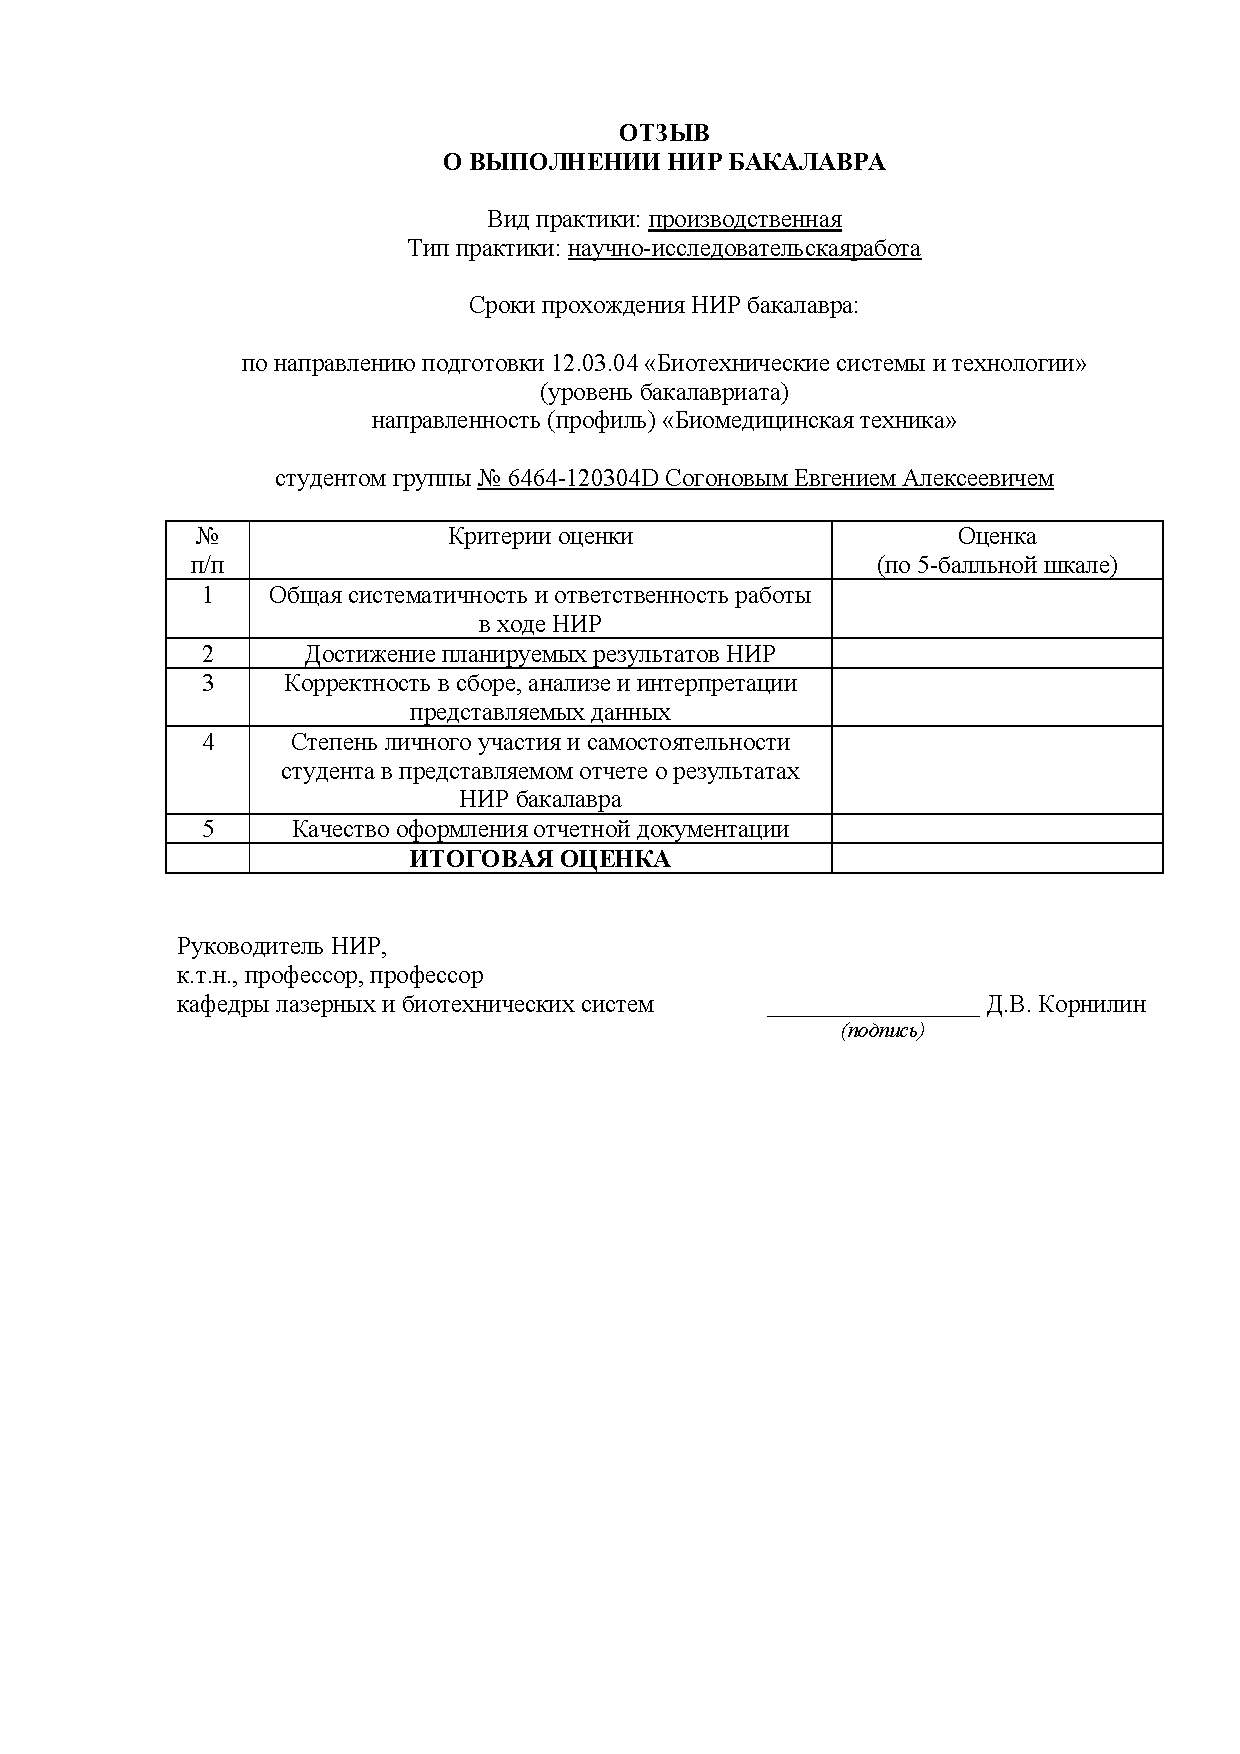
\includepdf[pages={-}]{2.pdf}

% \input{RefProject-base}% осн часть


%\begin{landscape}
% текст в альбомной ориентации
% (таблица, рисунок, схема и т. п.)
%\end{landscape}

% \likechapter{Вступление}






\end{document}